% Personal Finance Tracker — DATA 333 Project Report
% Build: python tools/build_latex.py   (or: latexmk -pdf -outdir=build Project_Report.tex)
\documentclass[11pt,letterpaper]{article}

\usepackage[T1]{fontenc}
\usepackage[utf8]{inputenc}
\usepackage{lmodern}
\usepackage[english]{babel}
\usepackage[margin=0.85in,headheight=14pt]{geometry}
\usepackage{microtype}
\usepackage{graphicx}
\usepackage{float}
\usepackage[font=small,labelfont=bf]{caption}
\usepackage{subcaption}
\usepackage{booktabs}
\usepackage{tabularx}
\usepackage{array}
\usepackage[table]{xcolor}
\usepackage{amssymb}
\usepackage{listings}
\usepackage{tikz}
\usetikzlibrary{positioning,arrows.meta,fit,backgrounds,calc}
\usepackage{fancyhdr}
\usepackage{enumitem}
\usepackage{needspace}
\usepackage[hidelinks]{hyperref}
\usepackage[capitalise,noabbrev]{cleveref}

\graphicspath{{../figures/}}
% Generated by tools/build_latex.py — do not edit by hand.
\newcommand{\StudentNameField}{\underline{\hspace{6cm}}}
\newcommand{\SubmissionDate}{October 1, 2026}
\newcommand{\TestCount}{[tests not run]}
\newcommand{\CoveragePct}{[coverage not measured]}
\newcommand{\SampleCount}{311}
\newcommand{\SampleFirstMonth}{2026-04}
\newcommand{\SampleLastMonth}{2026-09}
\newcommand{\VerPython}{3.11.16}
\newcommand{\VerTkinter}{8.6}
\newcommand{\VerPandas}{3.0.6}
\newcommand{\VerMatplotlib}{3.11.2}
\newcommand{\VerPlotly}{7.1.0}
\newcommand{\VerStreamlit}{1.64.0}
\newcommand{\VerPillow}{12.3.0}
\newcommand{\VerPythonPptx}{1.0.2}
\newcommand{\VerPythonDocx}{1.2.0}
\newcommand{\VerPlaywright}{1.63.0}
\newcommand{\VerRich}{15.0.0}
\newcommand{\VerPytest}{9.1.1}
\newcommand{\VerPytestCov}{7.1.0}
\newcommand{\VerRuff}{0.16.9}

% Shared code-listing style for the report and the memo.
% Code excerpts are extracted from the real source by tools/build_latex.py
% (docs/shared/generated/*.py); they are never copied by hand.
\definecolor{codebg}{HTML}{F6F8FA}
\definecolor{codeframe}{HTML}{D0D7DE}
\definecolor{codecomment}{HTML}{2E7D32}
\definecolor{codekeyword}{HTML}{1565C0}
\definecolor{codestring}{HTML}{A0522D}
\lstdefinestyle{project}{
  language=Python,
  basicstyle=\ttfamily\footnotesize,
  keywordstyle=\color{codekeyword}\bfseries,
  commentstyle=\color{codecomment}\itshape,
  stringstyle=\color{codestring},
  backgroundcolor=\color{codebg},
  frame=single, rulecolor=\color{codeframe},
  framesep=3pt, xleftmargin=4pt, xrightmargin=4pt,
  breaklines=true, breakatwhitespace=true,
  postbreak=\mbox{\textcolor{codeframe}{$\hookrightarrow$}\space},
  columns=fullflexible, keepspaces=true,
  showstringspaces=false, tabsize=4,
  upquote=true,
  aboveskip=4pt, belowskip=4pt,
  % pdflatex + listings cannot read multi-byte UTF-8 characters directly:
  % map every non-ASCII character used in the excerpts to a LaTeX equivalent.
  literate=
    {—}{{---}}1 {–}{{--}}1 {→}{{$\rightarrow$}}1 {·}{{$\cdot$}}1
    {✓}{{\checkmark}}1 {✗}{{$\times$}}1 {█}{{\rule{0.5em}{0.7em}}}1
    {💰}{{\$}}1 {é}{{\'e}}1 {è}{{\`e}}1 {à}{{\`a}}1 {ê}{{\^e}}1 {ç}{{\c{c}}}1
    {⚠}{{!}}1 {…}{{...}}1 {─}{{-}}1
}
\lstset{style=project}


\definecolor{accent}{HTML}{1565C0}
\definecolor{muted}{HTML}{5F6B66}
\newcommand{\code}[1]{\texttt{#1}}
\newcolumntype{Y}{>{\raggedright\arraybackslash}X}
\setlength{\parskip}{3pt}
\setlength{\parindent}{0pt}
\captionsetup[sub]{font=footnotesize}
\setlist{nosep,leftmargin=1.2em}

\pagestyle{fancy}
\fancyhf{}
\fancyhead[L]{\small\color{muted}Personal Finance Tracker --- DATA 333 Project Report}
\fancyhead[R]{\small\color{muted}Bellevue College}
\fancyfoot[C]{\small\thepage}
\renewcommand{\headrulewidth}{0.4pt}

\hypersetup{
  pdftitle={Personal Finance Tracker --- DATA 333 Project Report},
  pdfsubject={DATA 333 -- Data Management \& Analysis, Bellevue College},
}

\begin{document}

% ------------------------------------------------------------------ title page
\begin{titlepage}
  \centering
  \vspace*{3.2cm}
  {\Huge\bfseries\color{accent} Personal Finance Tracker\par}
  \vspace{0.4cm}
  {\LARGE DATA 333 Project Report\par}
  \vspace{1.2cm}
  {\large A Python application to track, analyze and visualize personal finances\\
   with pandas, Tkinter and Streamlit\par}
  \vspace{2.2cm}
  {\large DATA 333 -- Data Management \& Analysis\par}
  \vspace{0.2cm}
  {\large Bellevue College --- Prior Learning Assessment (PLA)\par}
  \vspace{2.4cm}
  {\large Student Name: \StudentNameField\par}
  \vspace{0.6cm}
  {\large \SubmissionDate\par}
  \vfill
  {\small\color{muted} Source code, data and build scripts:
   \url{https://github.com/14juanito/Personal-finance-tracker}\par}
\end{titlepage}

% ------------------------------------------------------------------ 1
\section{Project overview and objectives}
The Personal Finance Tracker records income and expenses, organizes them into categories,
and turns them into summaries, trends, budget alerts and savings-goal progress. One tested
core is used by three interfaces: an interactive \textbf{console menu}
(\code{python main.py cli}), a \textbf{Tkinter desktop application}
(\code{python main.py gui}) and an interactive \textbf{Streamlit dashboard}
(\code{streamlit run finance\_tracker/dashboard.py}). A non-interactive \textbf{demo
mode} (\code{python main.py demo}) runs every feature on a reproducible sample of
\SampleCount{} fictional transactions (\SampleFirstMonth{} to \SampleLastMonth).
\textbf{Requires Python 3.11+.}

The objectives, taken from the course brief, were to: track income and expenses;
categorize transactions; display spending summaries; set and track savings goals; save and
load data from files; analyze spending trends; visualize the results --- while
demonstrating every core concept of the course (input/output, decisions and loops,
functions, files and exceptions, lists/dictionaries/sets, classes, pandas) and implementing
all four enhancements: Tkinter GUI, JSON \emph{and} CSV storage, budget alerts and a
Streamlit dashboard.

% ------------------------------------------------------------------ 2
\section{Key features}
\begin{itemize}
  \item \textbf{Transactions} --- add, edit, delete, text search and filters (kind,
        category, date range, amount); every value is validated before it is stored.
  \item \textbf{Summaries and trends} --- monthly income, expenses, net and savings rate,
        category shares, a 3-month rolling average, month-over-month change, top expenses.
  \item \textbf{Budgets and alerts} --- a monthly limit per category; \emph{WARNING} at
        80\,\%, \emph{EXCEEDED} at 100\,\%, raised as soon as a new expense crosses a limit.
  \item \textbf{Savings goals} --- target, deadline, contributions and milestones at
        25/50/75/100\,\%.
  \item \textbf{Files} --- full state in JSON, transactions in CSV (import/export), atomic
        writes, and recovery from a corrupted file.
\end{itemize}
All figures below are real captures of the running application on the sample data, produced
by \code{tools/capture\_screenshots.py}; GUI and dashboard captures are cropped to the region
being discussed (full-size images are in \code{docs/figures/}).

\begin{figure}[H]
  \centering
  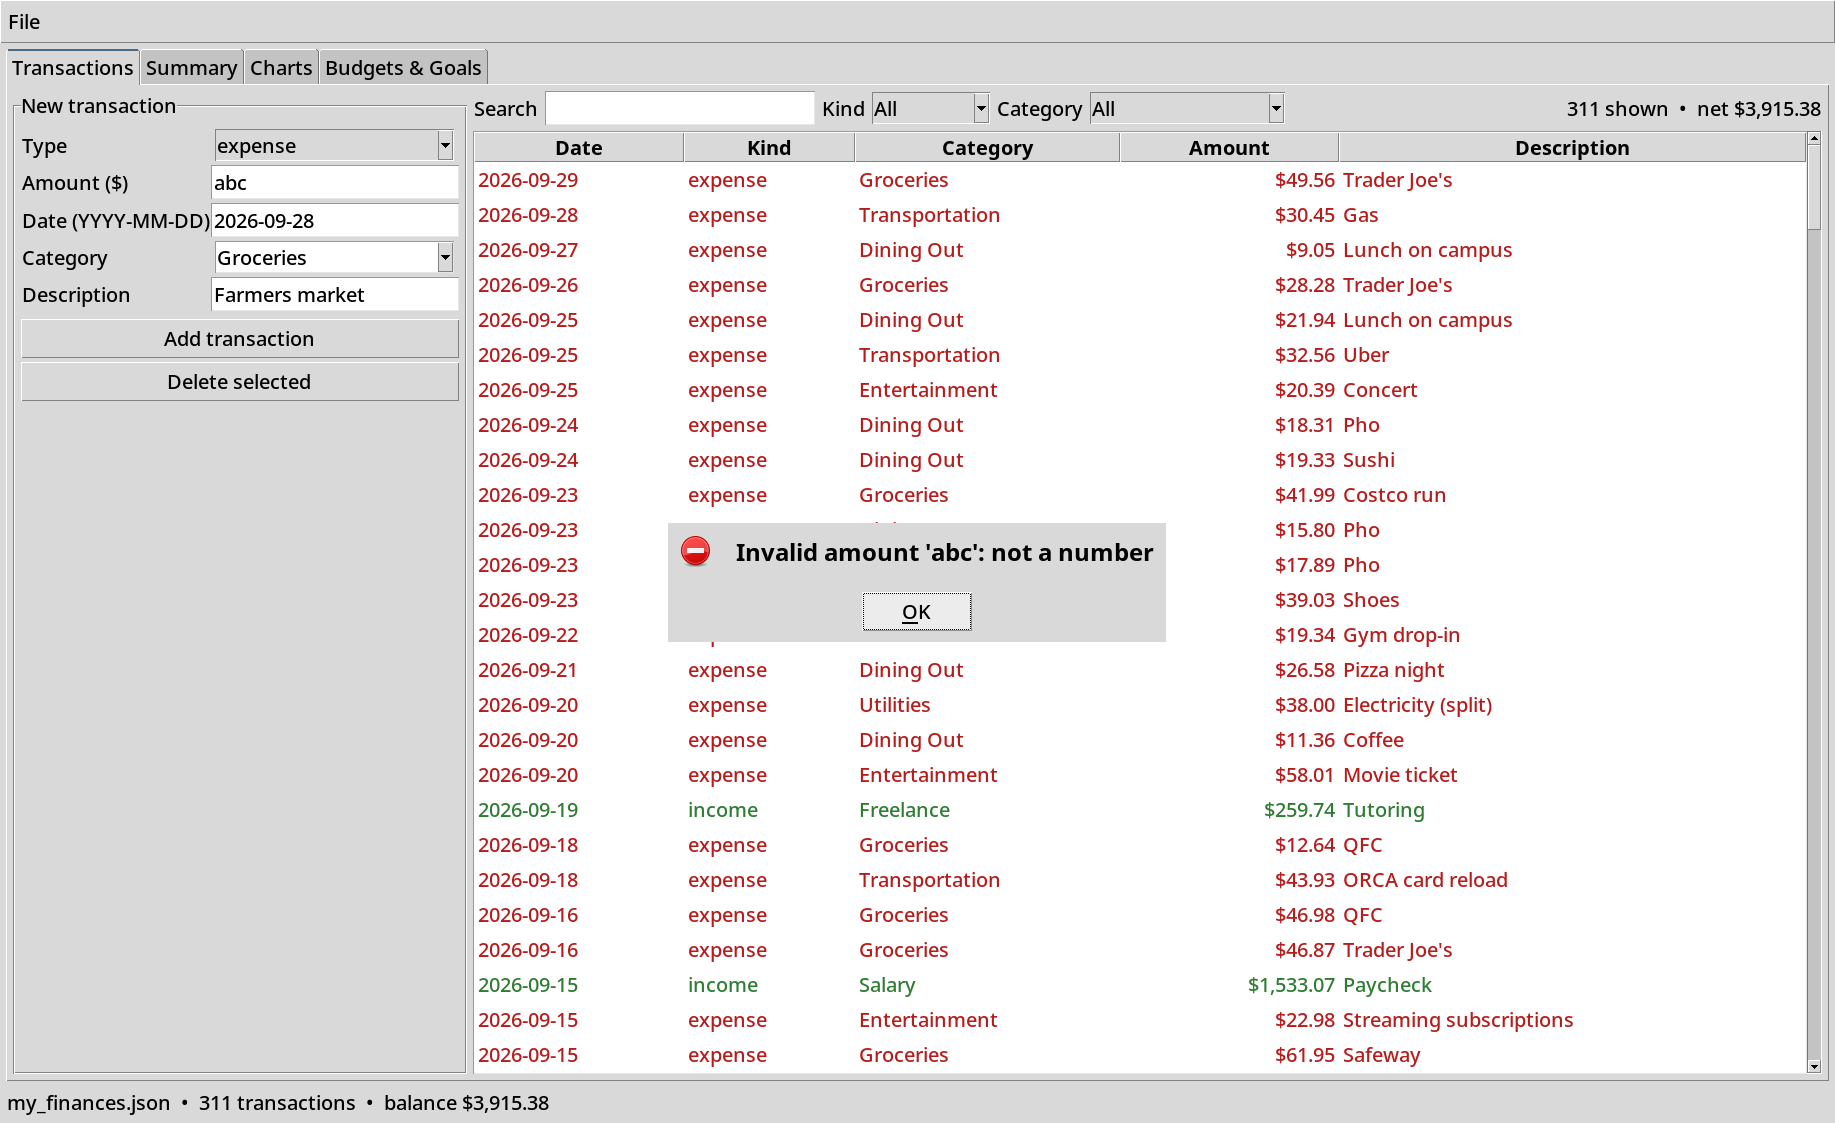
\includegraphics[width=0.76\linewidth,trim=0 212.6 280.8 0,clip]{gui_validation_error.png}
  \caption{Tkinter desktop application (\code{python main.py gui}): the entry form, the
  searchable and sortable transaction table, and the message shown when an invalid amount
  (\code{abc}) is submitted --- nothing is stored.}
  \label{fig:gui}
\end{figure}

\begin{figure}[H]
  \centering
  \begin{subfigure}{0.495\linewidth}
    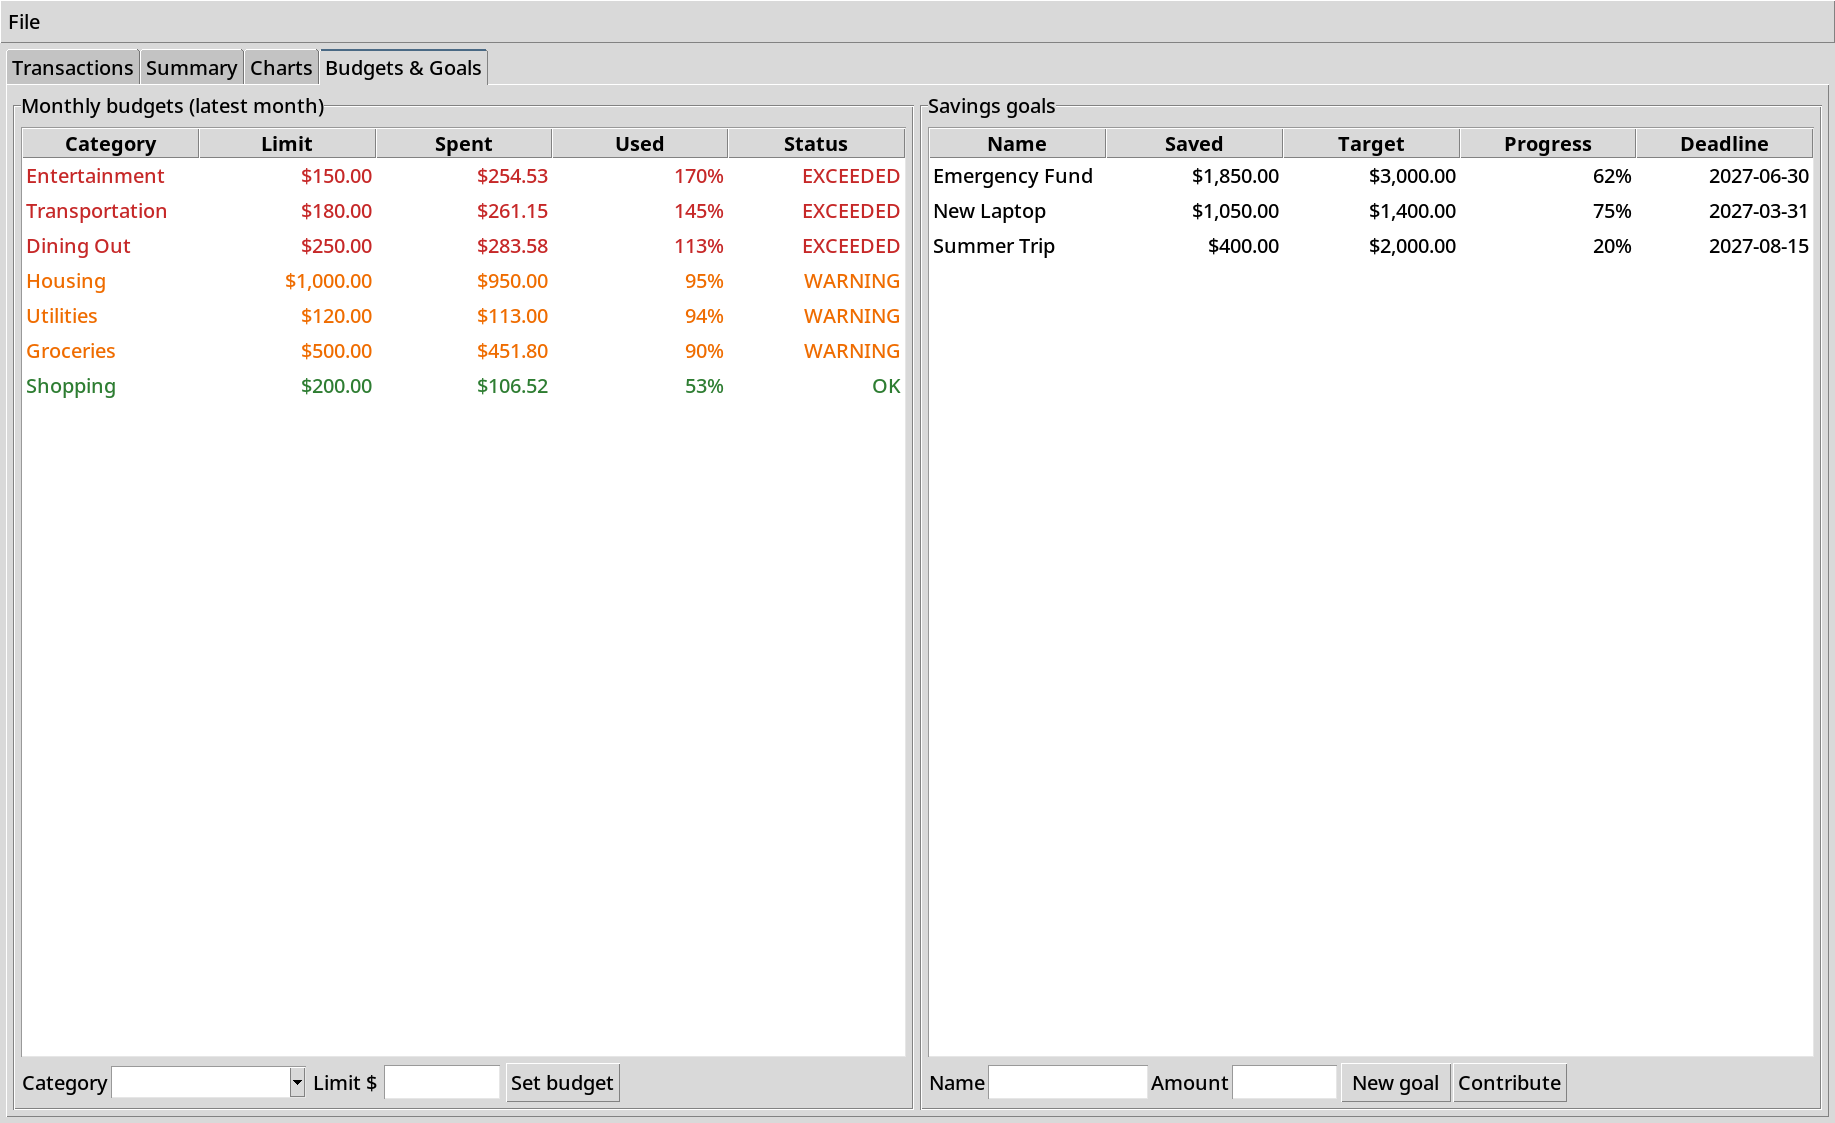
\includegraphics[width=\linewidth,trim=0 313.4 434.4 19.2,clip]{gui_budgets_alerts.png}
    \caption{Budgets with EXCEEDED (red) and WARNING (orange) rows.}
    \label{fig:gui-budgets}
  \end{subfigure}\hfill
  \begin{subfigure}{0.495\linewidth}
    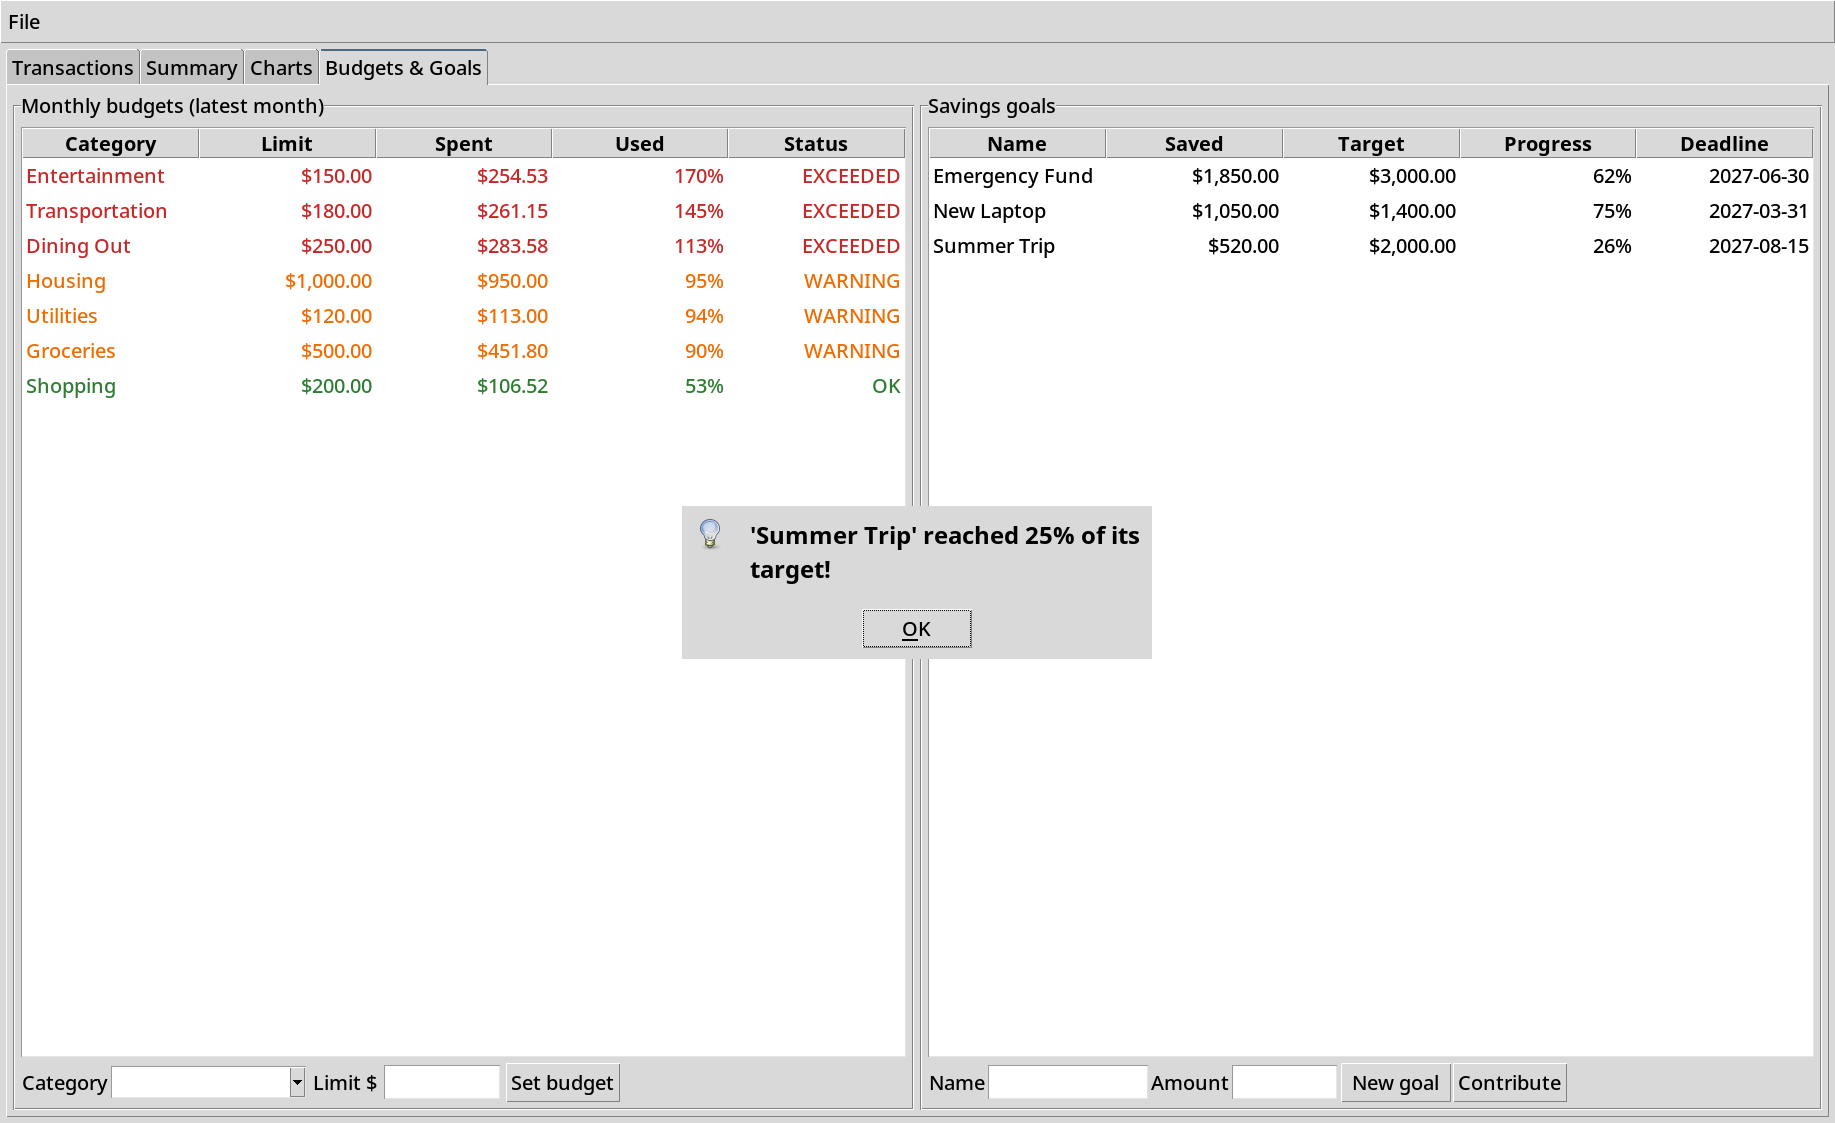
\includegraphics[width=\linewidth,trim=288 212.6 0 19.2,clip]{gui_savings_goals.png}
    \caption{A contribution crosses the 25\,\% milestone of a goal.}
    \label{fig:gui-goals}
  \end{subfigure}
  \caption{Budget alerts and savings goals in the Tkinter application.}
  \label{fig:gui-alerts}
\end{figure}

\begin{figure}[H]
  \centering
  \begin{subfigure}{0.495\linewidth}
    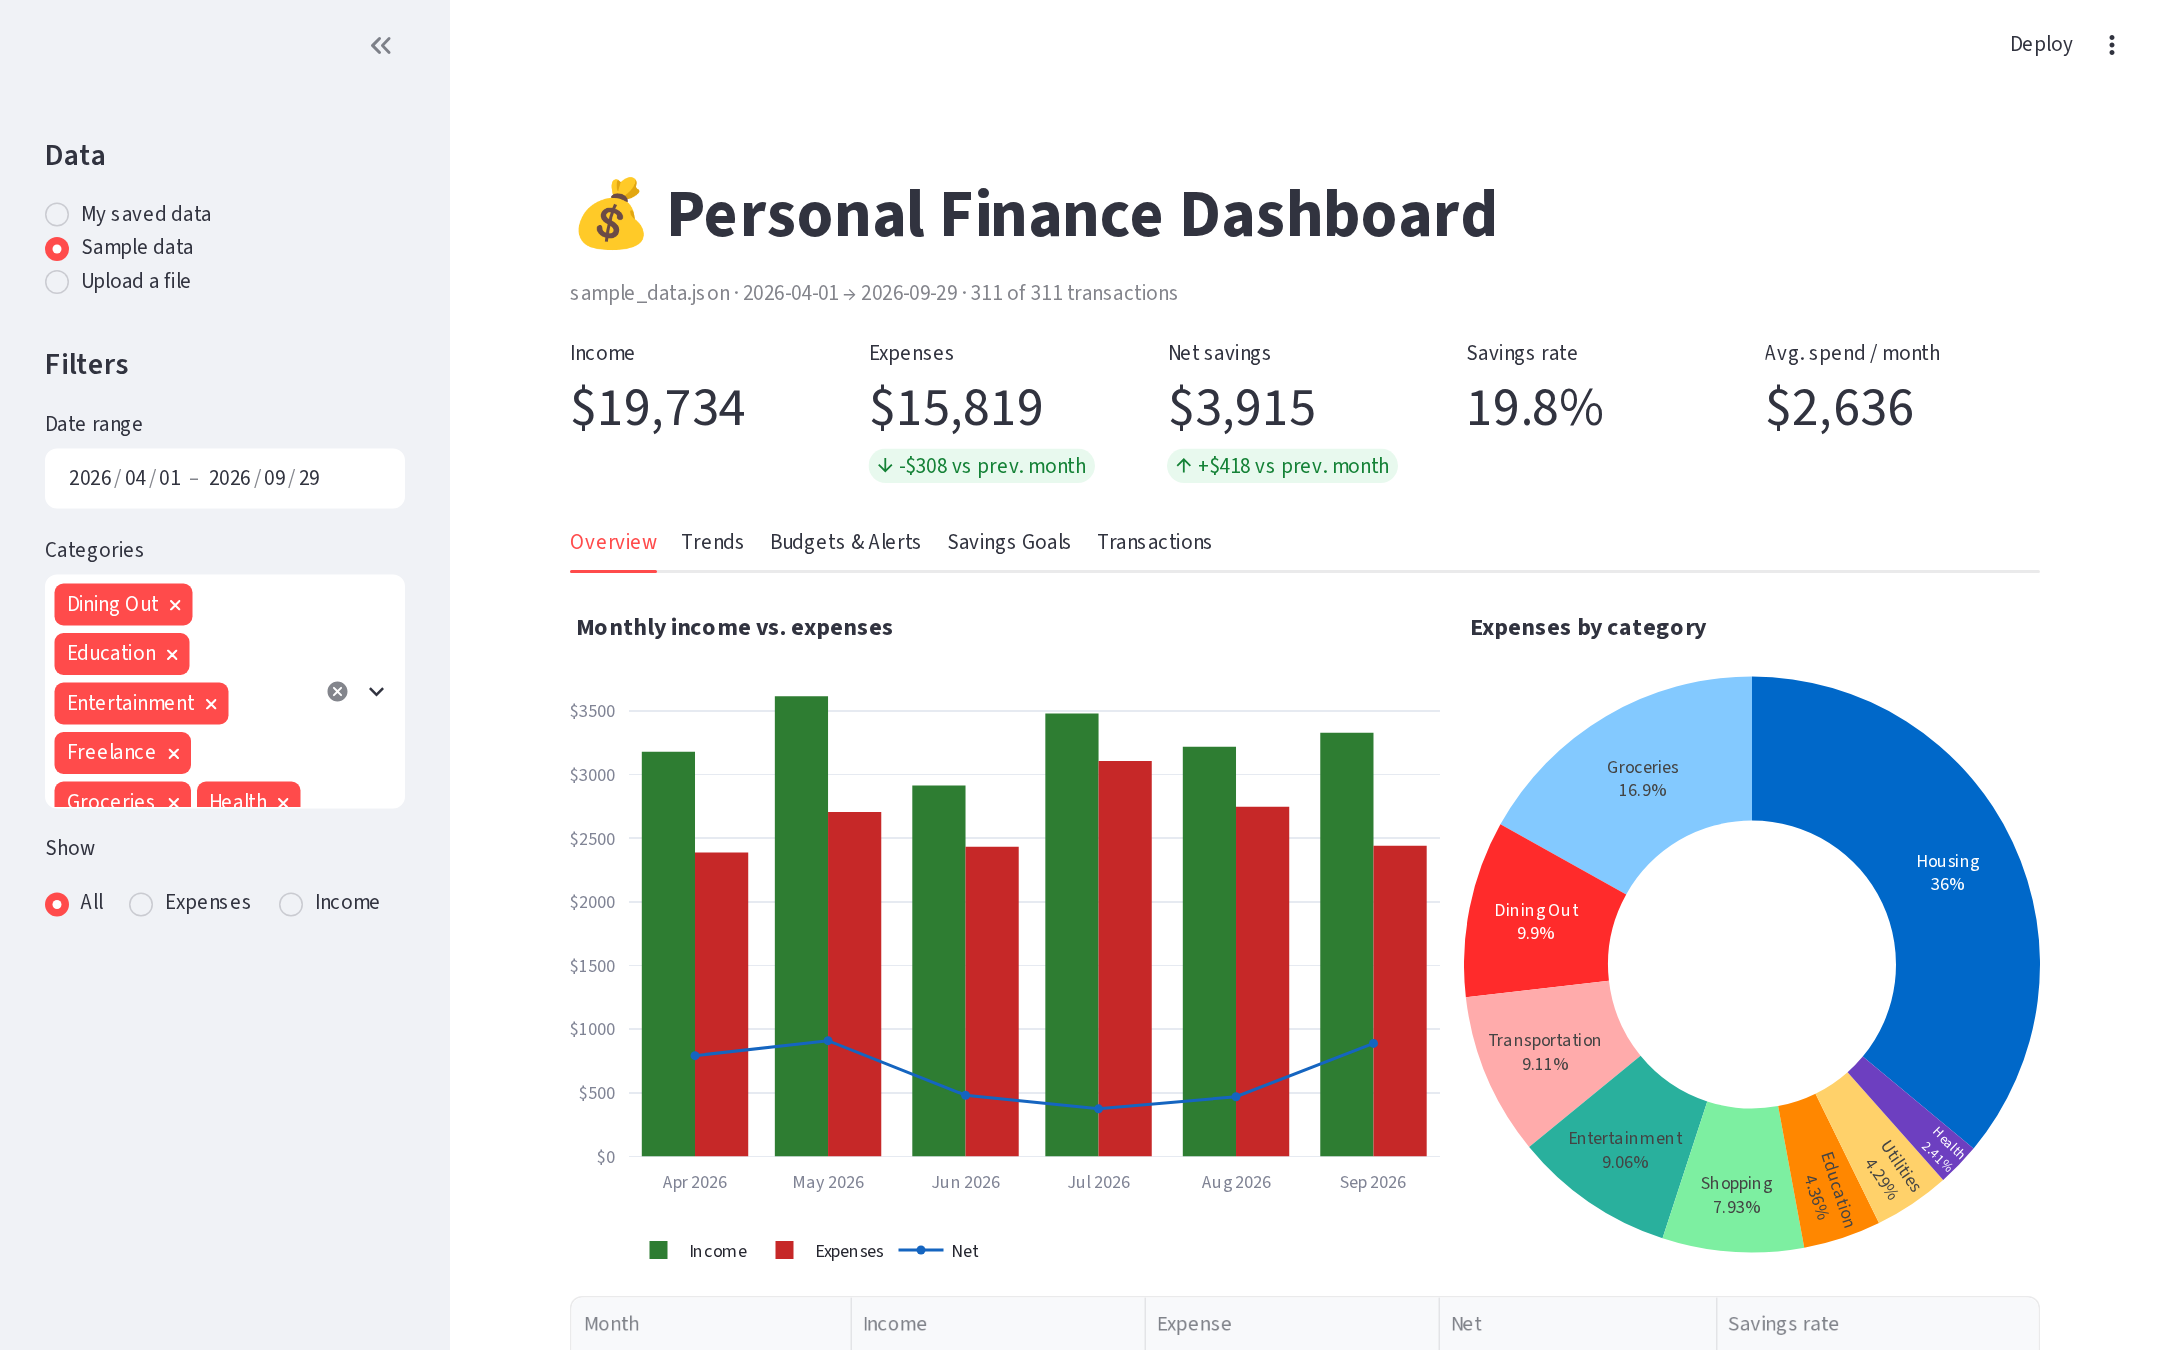
\includegraphics[width=\linewidth,trim=230.4 72 0 52.8,clip]{dashboard_overview.png}
    \caption{KPIs with month-over-month deltas, Plotly charts.}
    \label{fig:dash-overview}
  \end{subfigure}\hfill
  \begin{subfigure}{0.495\linewidth}
    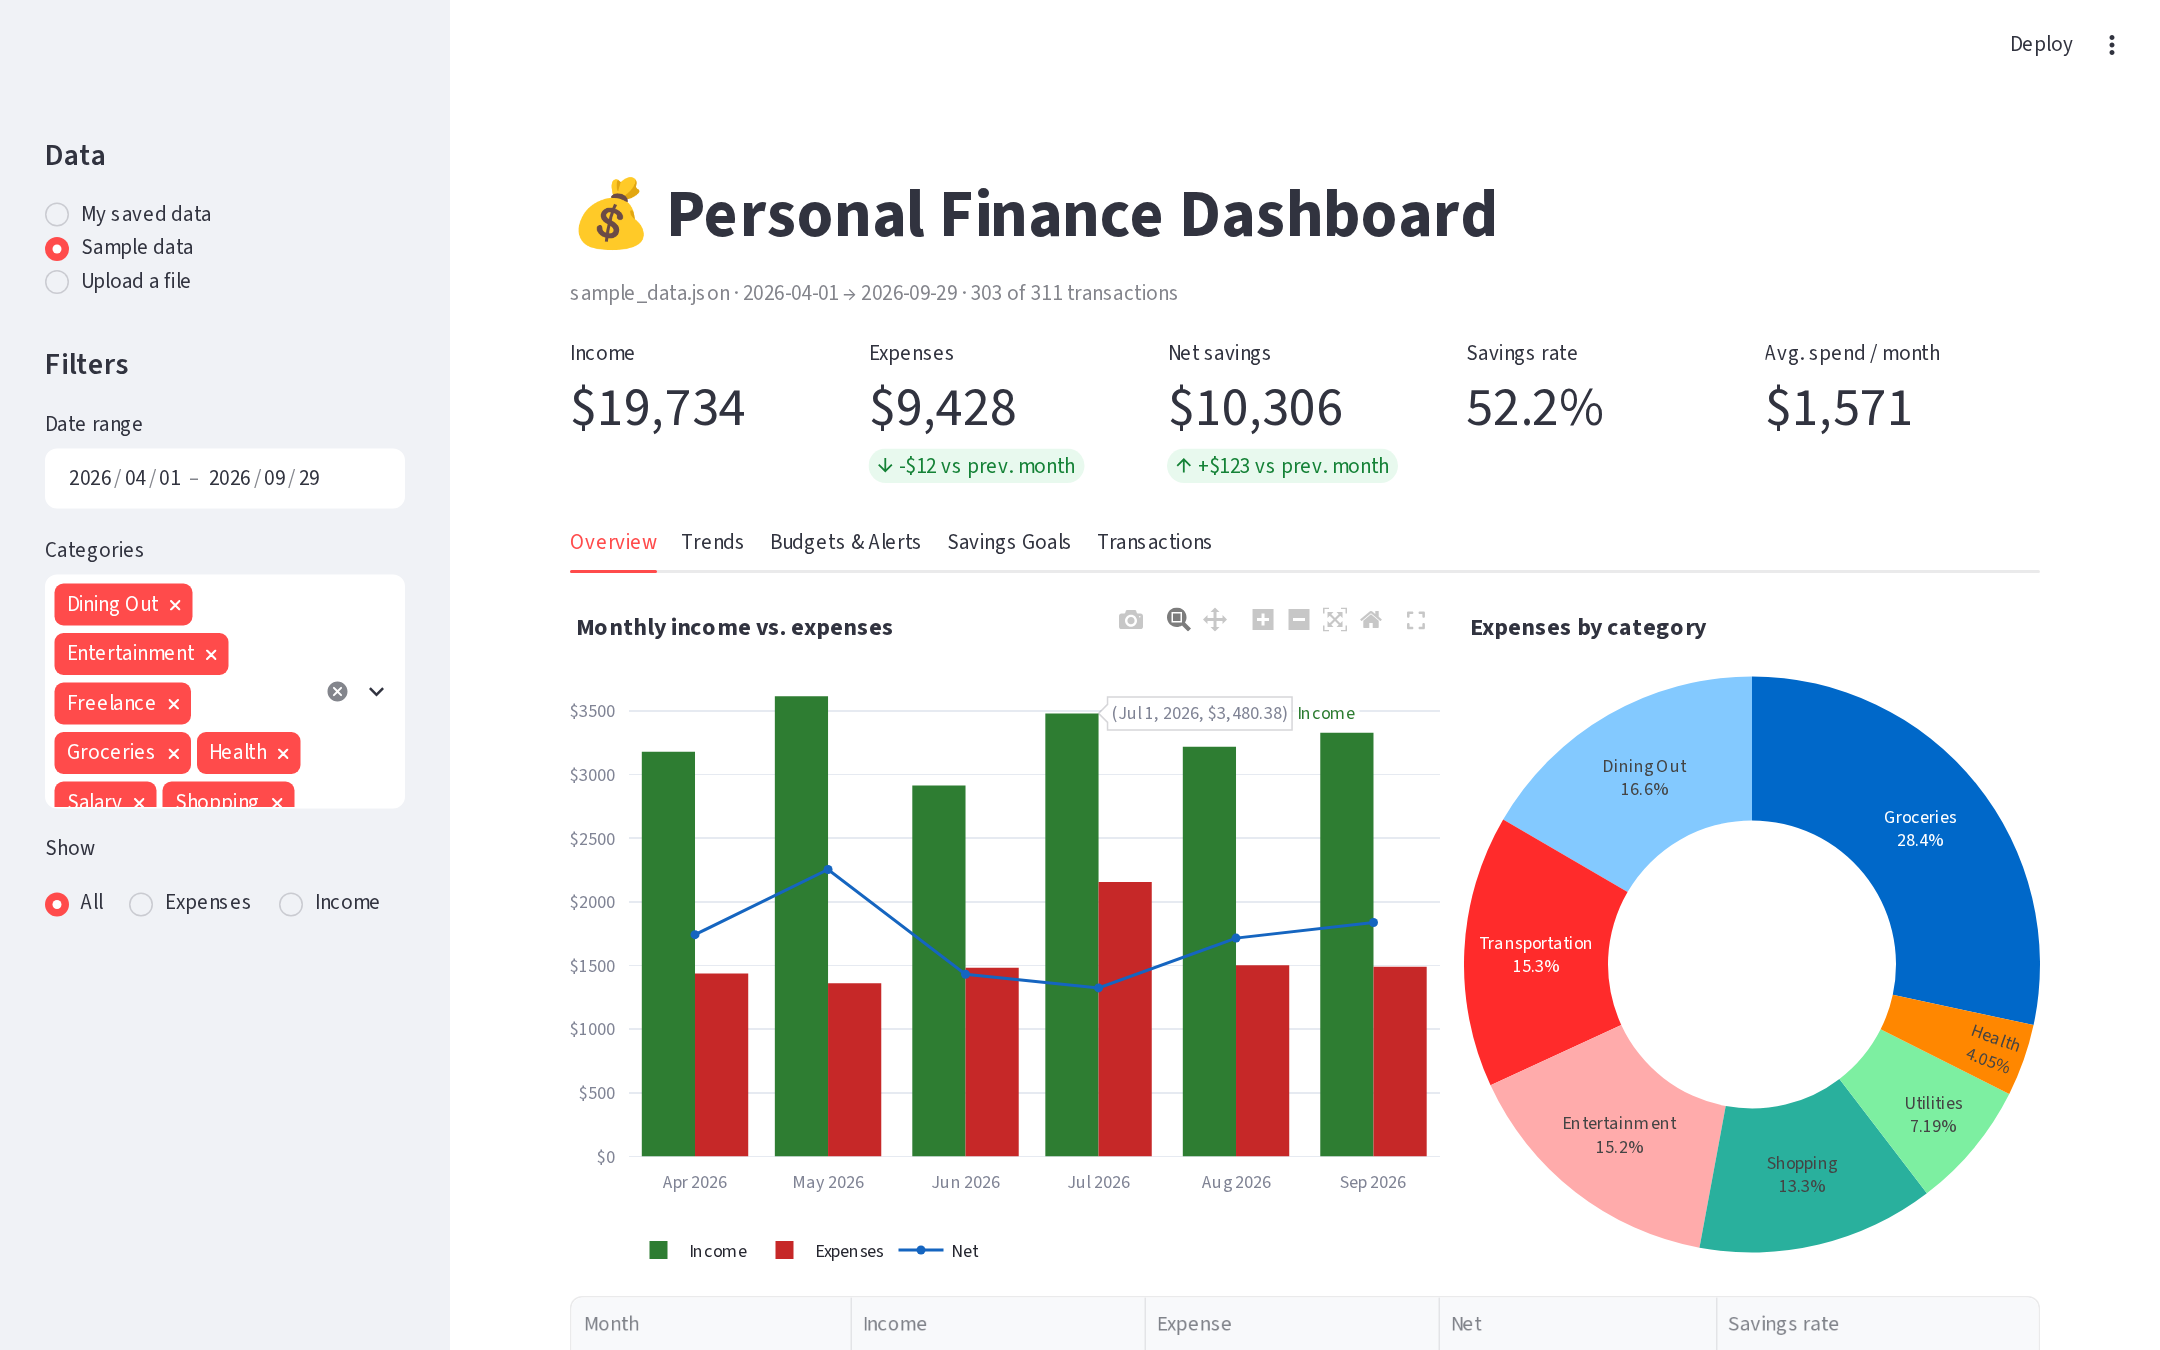
\includegraphics[width=\linewidth,trim=230.4 72 288 268.8,clip]{dashboard_interactive.png}
    \caption{Hovering a bar shows its exact value (Plotly tooltip).}
    \label{fig:dash-interactive}
  \end{subfigure}
  \caption{Streamlit dashboard, captured with headless Chromium (Playwright).}
  \label{fig:dashboard}
\end{figure}

\begin{figure}[H]
  \centering
  \begin{subfigure}[t]{0.495\linewidth}
    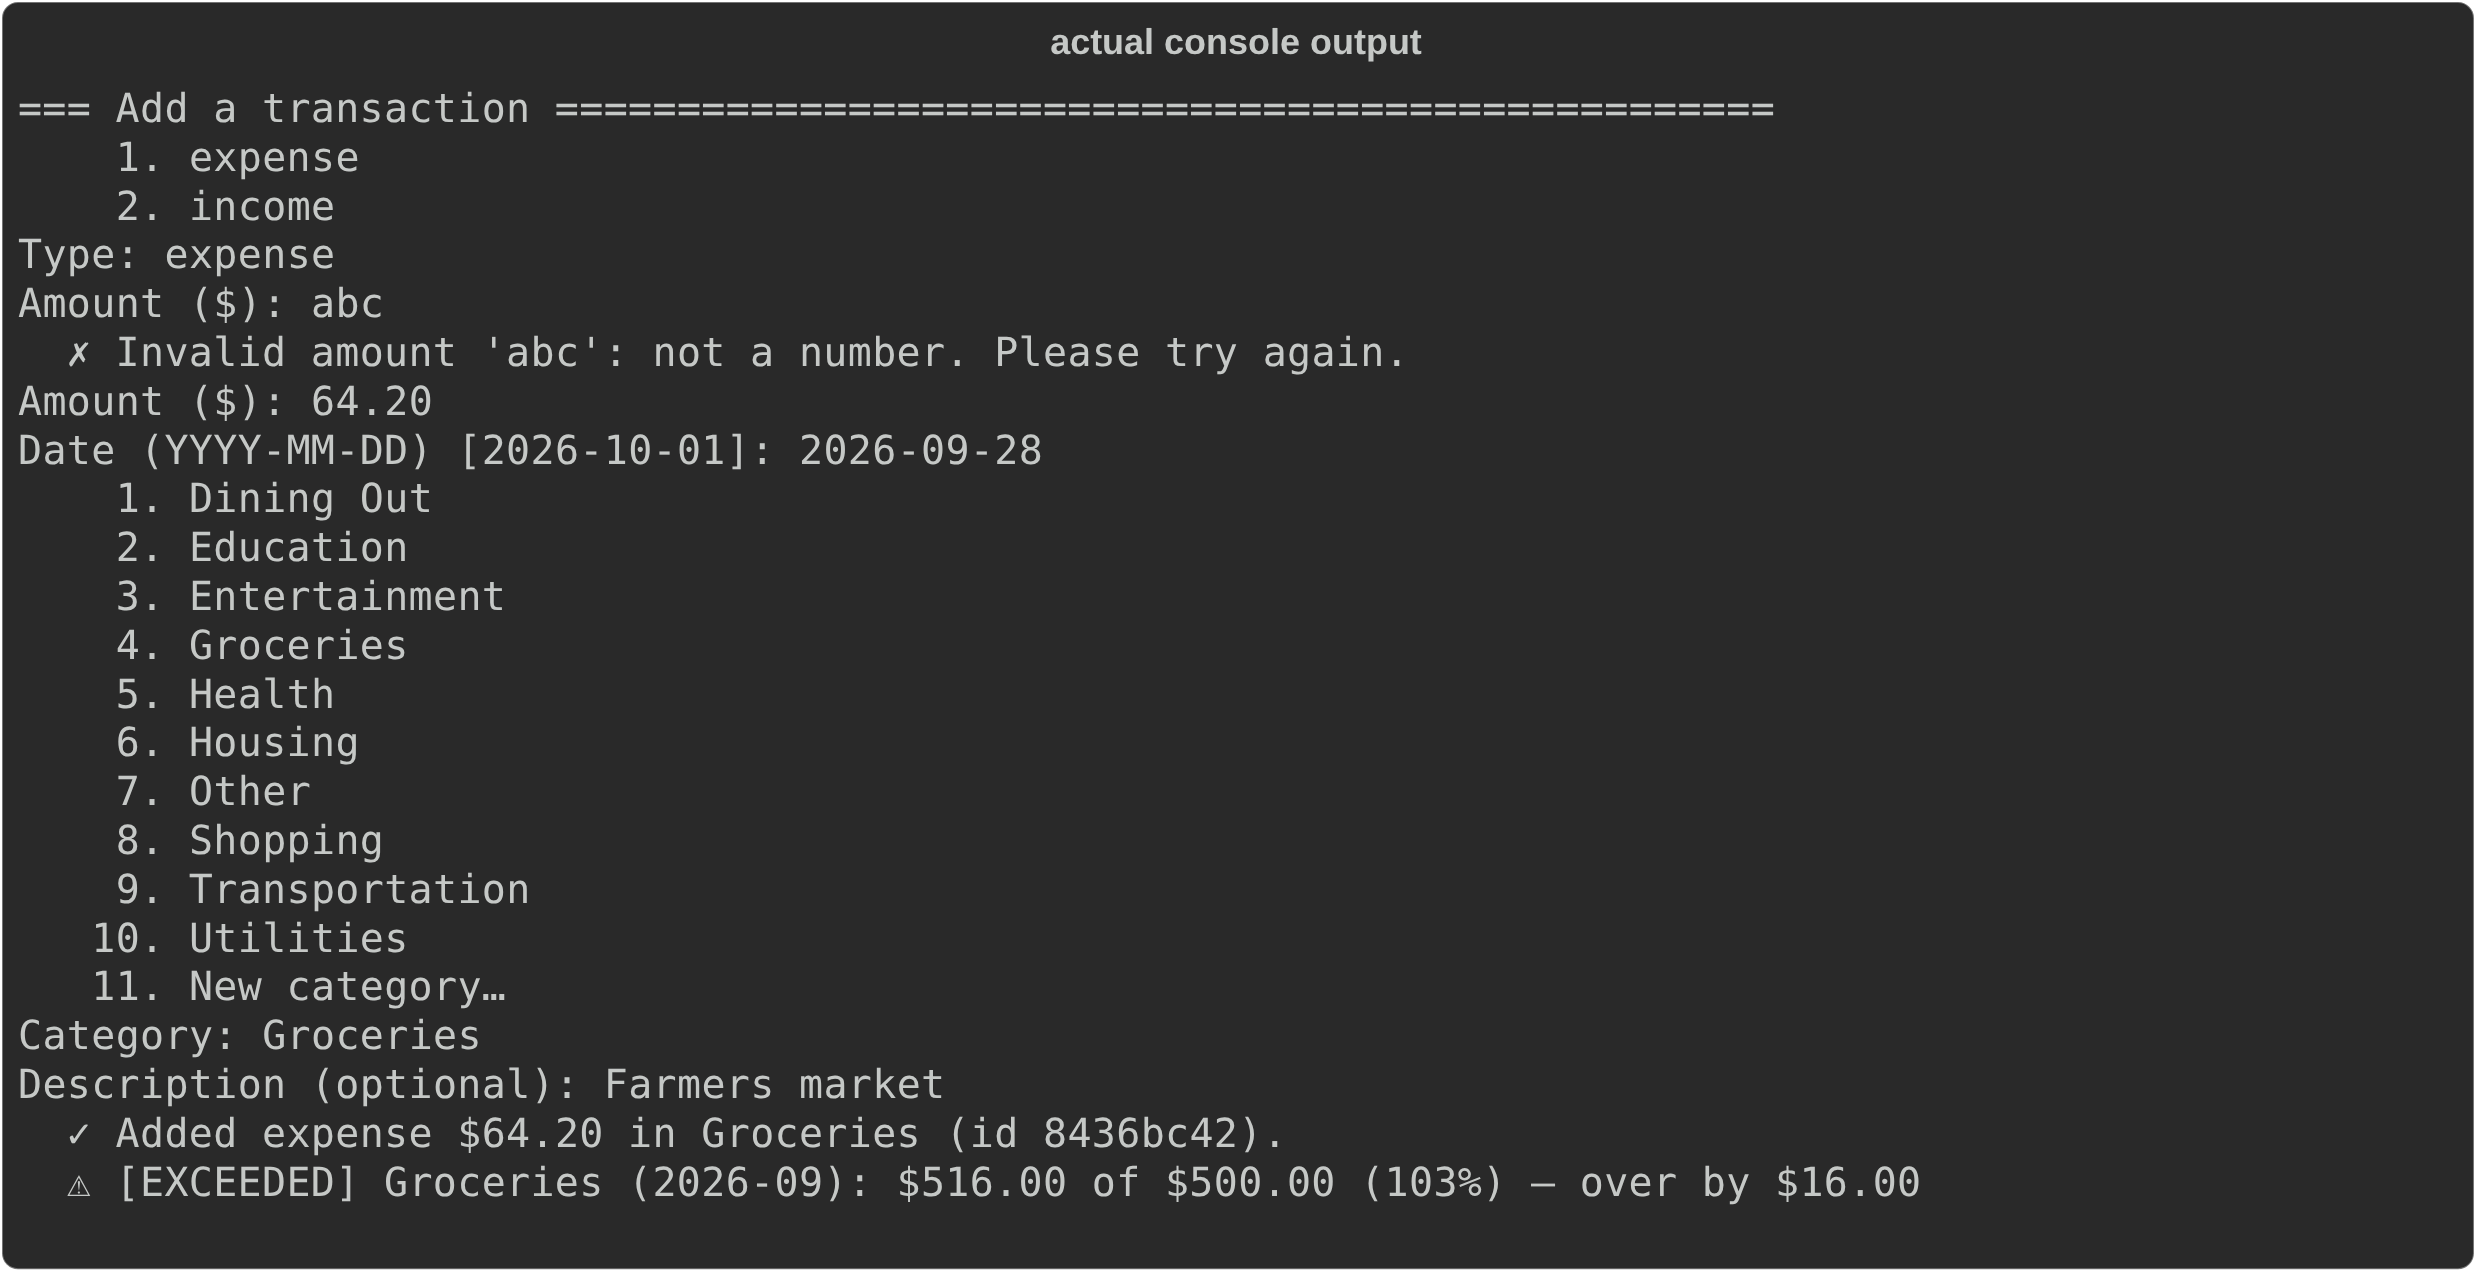
\includegraphics[width=\linewidth]{cli_session_add.png}
    \caption{\code{python main.py cli}: re-prompt, then budget alert.}
    \label{fig:cli-add}
  \end{subfigure}\hfill
  \begin{subfigure}[t]{0.495\linewidth}
    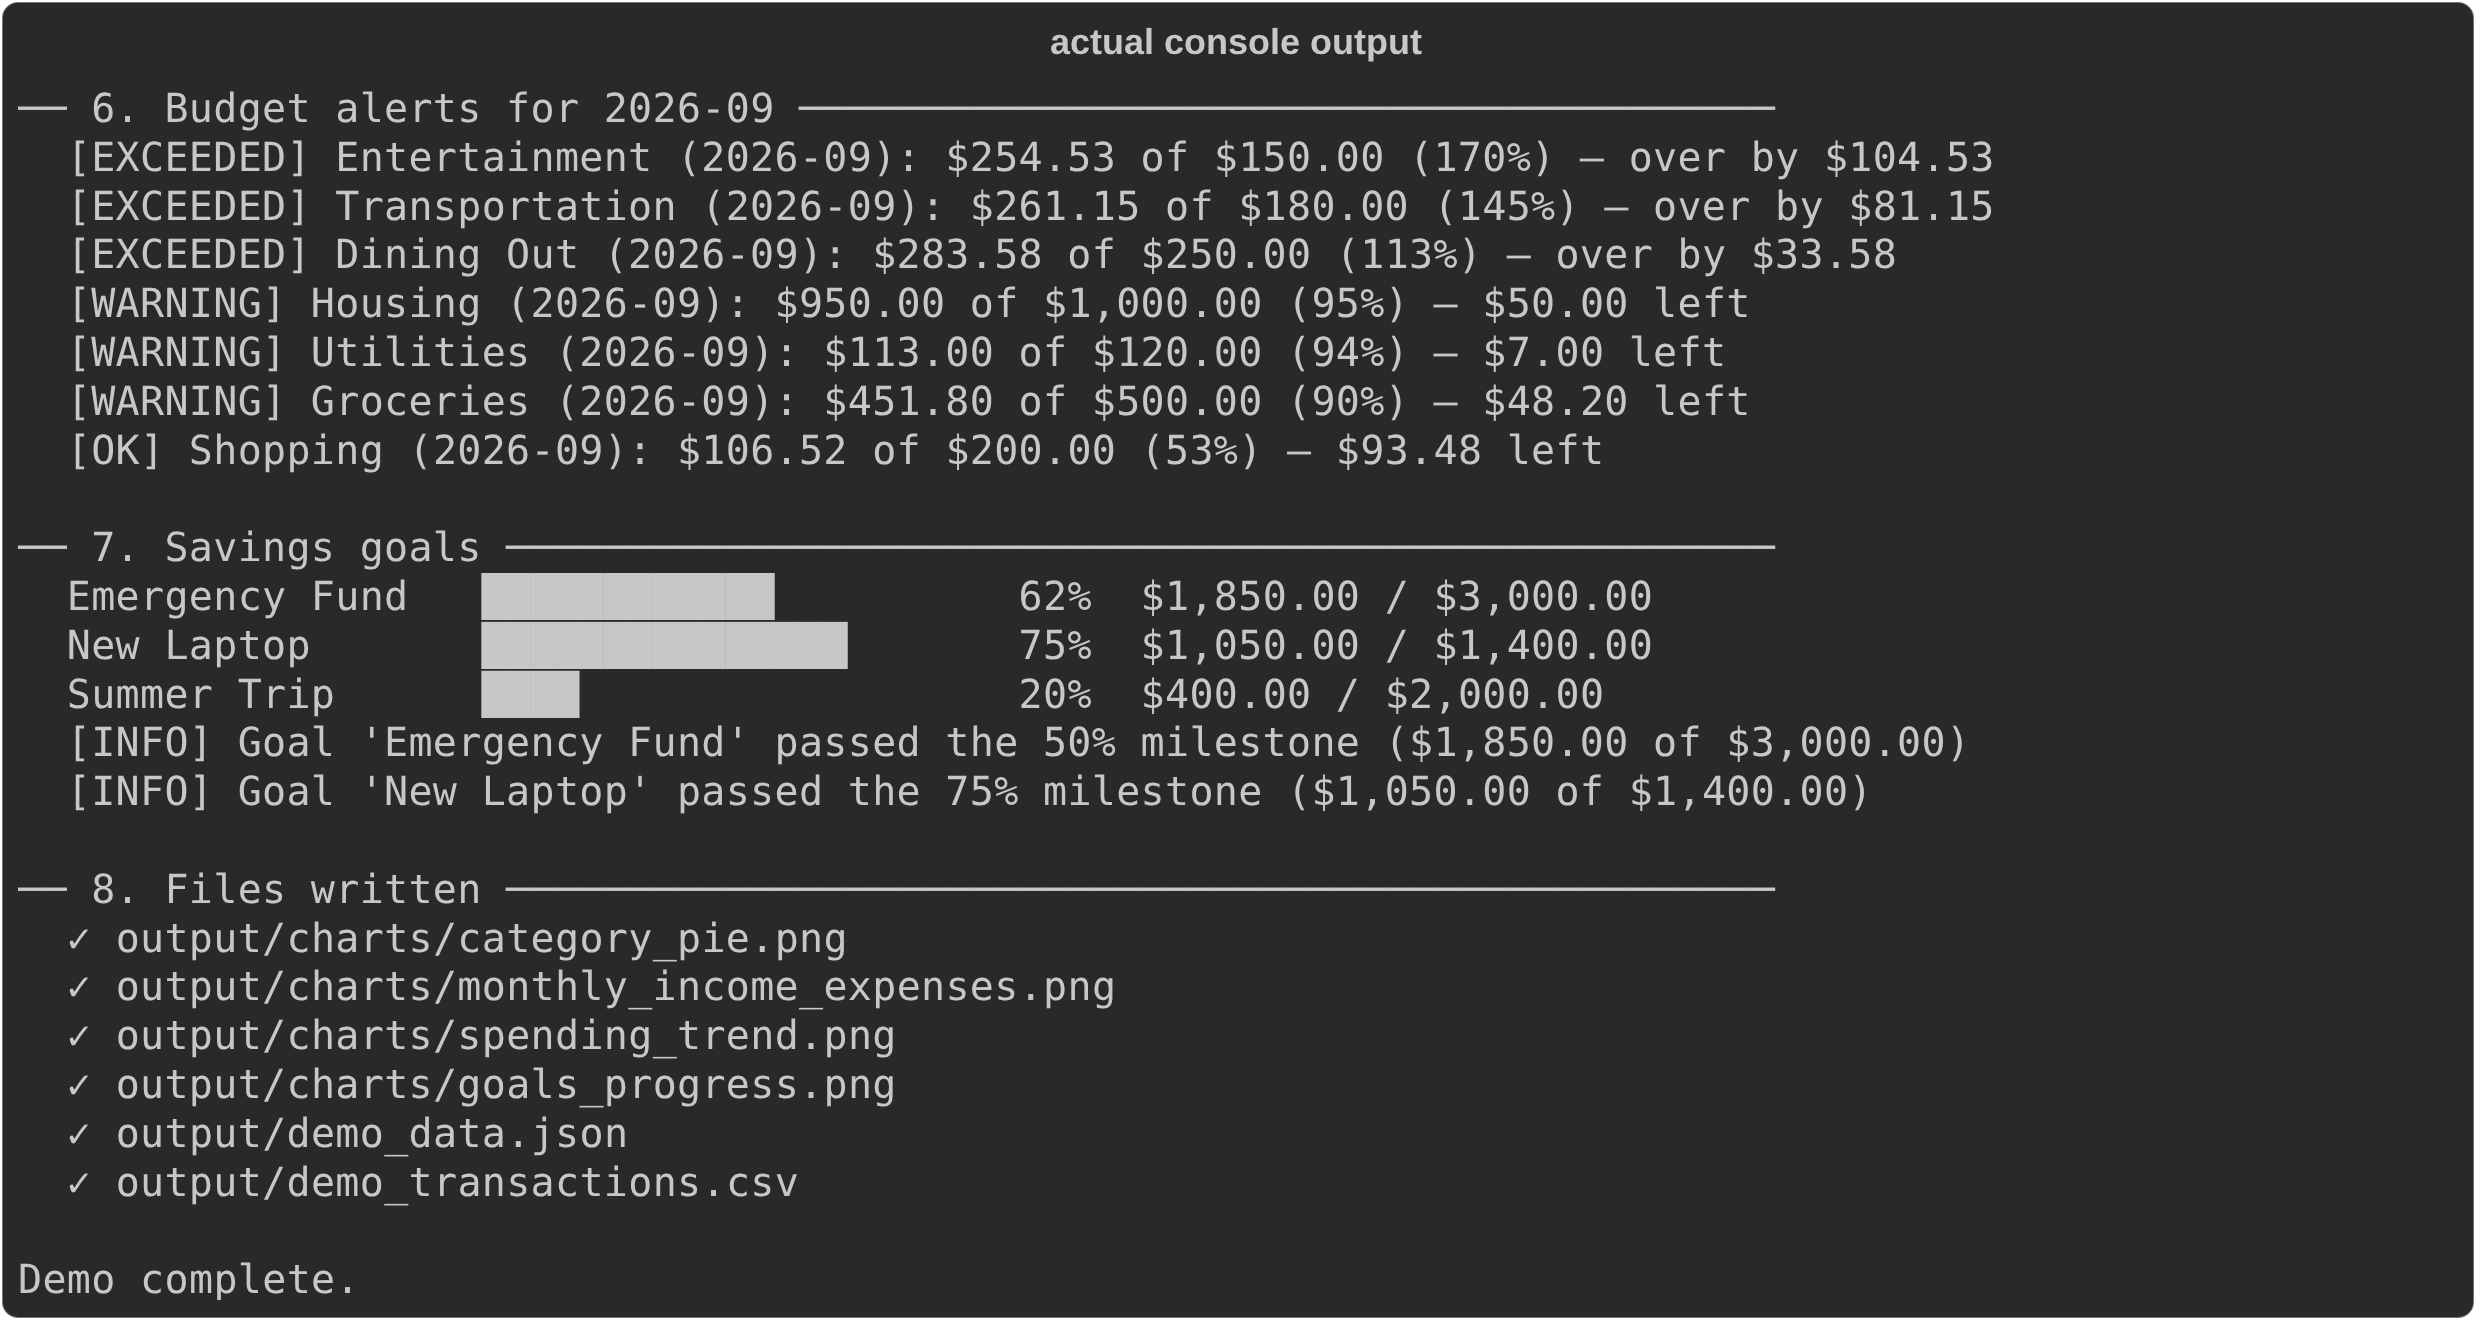
\includegraphics[width=\linewidth]{cli_demo_alerts.png}
    \caption{\code{python main.py demo}: alerts, goals, files written.}
    \label{fig:cli-demo}
  \end{subfigure}
  \caption{Console modes --- actual console output, recorded with \code{rich}.}
  \label{fig:cli}
\end{figure}

\Cref{fig:gui,fig:gui-alerts} show the desktop application, \cref{fig:dashboard} the
web dashboard and \cref{fig:cli} the two console modes; the same alerts appear in all three
interfaces because they come from the same functions.

% ------------------------------------------------------------------ 3
\section{How course concepts were applied}
Every concept is tagged in the source with a \code{\# Concept:} comment at the exact line
where it is applied; a test (\code{tests/test\_code\_standards.py}) fails if one is missing.

{\small
\begin{tabularx}{\linewidth}{@{}>{\raggedright\arraybackslash}p{2.45cm}>{\raggedright\arraybackslash}p{4.8cm}Y@{}}
\toprule
\textbf{Concept} & \textbf{File / function} & \textbf{Excerpt} \\
\midrule
Input / output & \code{cli.py} -- \code{ConsoleApp.ask}, \code{show\_summary} &
  \code{self.\_input(prompt).strip()}; aligned f-string tables \\
Decisions \& loops & \code{alerts.budget\_level}, \code{ConsoleApp.run}, \code{prompt\_amount} &
  \code{if ratio >= EXCEEDED\_THRESHOLD: ... elif ...}; \code{while True:} re-prompt \\
Functions & \code{models.parse\_amount}, \code{analytics.*} &
  small, typed, documented functions reused by every interface \\
Files \& exceptions & \code{storage.load\_json}, \code{\_atomic\_write} &
  \code{try/except/else}; \code{try/except/finally}; corrupted file backed up \\
Lists / dicts / sets & \code{FinanceTracker.\_\_init\_\_} &
  \code{transactions: list}, \code{budgets: dict}, \code{categories: set} \\
Classes (OOP) & \code{Transaction}, \code{SavingsGoal}, \code{Budget}, \code{FinanceTracker} &
  dataclasses validated in \code{\_\_post\_init\_\_}; properties; inheritance \\
pandas & \code{analytics.monthly\_summary}, \code{spending\_trend} &
  \code{pivot\_table}, \code{groupby().agg()}, \code{rolling(3).mean()}, \code{pct\_change()} \\
\bottomrule
\end{tabularx}}

\vspace{4pt}
Three excerpts, extracted automatically from the real code (docstrings omitted):

\begin{minipage}[t]{0.485\linewidth}
\lstinputlisting[caption={\code{cli.py} --- loop, decision, exception},
  label=lst:prompt]{../shared/generated/prompt_amount.py}
\lstinputlisting[caption={\code{alerts.py} --- decision structure},
  label=lst:level]{../shared/generated/budget_level.py}
\end{minipage}\hfill
\begin{minipage}[t]{0.485\linewidth}
\lstinputlisting[caption={\code{analytics.py} --- pandas groupby},
  label=lst:pandas]{../shared/generated/category_breakdown.py}
\end{minipage}

% ------------------------------------------------------------------ 4
\section{Architecture}
The interfaces contain no business rules: they call \code{FinanceTracker} and the
\code{analytics}, \code{alerts} and \code{visualize} modules, and only format the results.
Validation lives in the model classes and every file format lives in \code{storage.py}.
\Cref{fig:architecture} shows the modules and how data flows between them.

\begin{figure}[H]
\centering
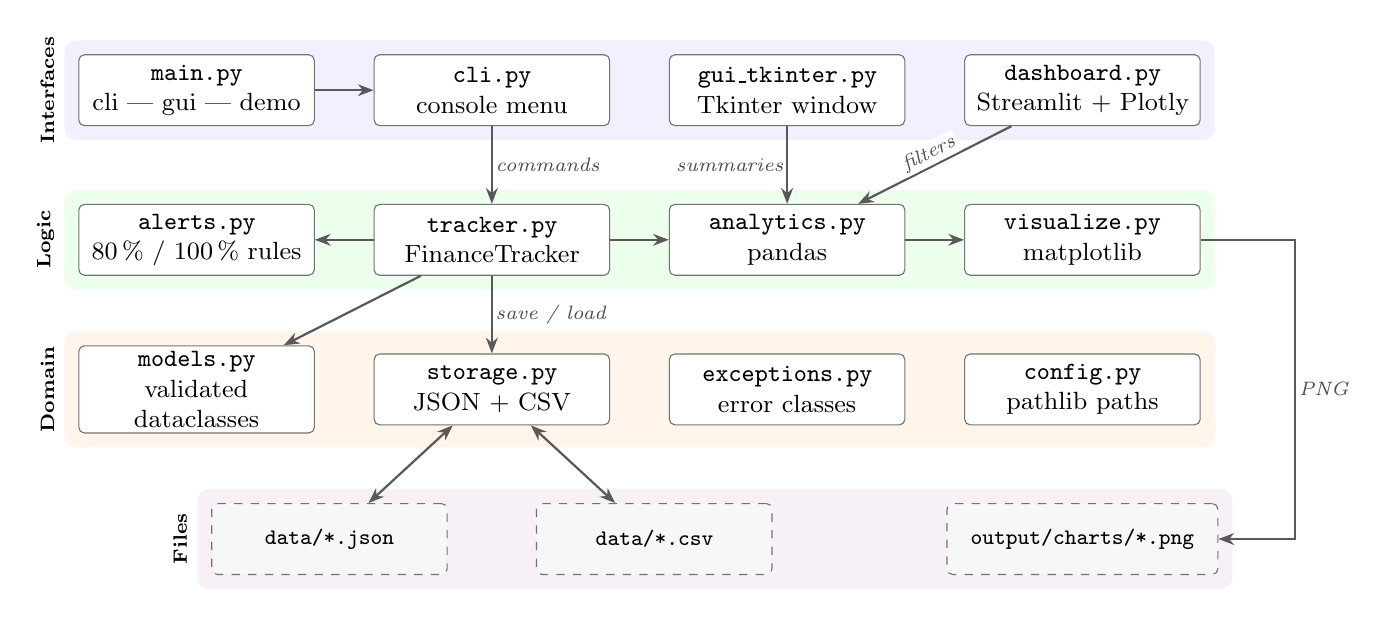
\begin{tikzpicture}[
  font=\small,
  mod/.style={draw=black!55, rounded corners=2pt, fill=white, align=center,
              minimum height=9mm, text width=2.85cm, inner sep=2pt},
  file/.style={mod, fill=black!3, dashed, text width=2.85cm, font=\footnotesize},
  flow/.style={-{Stealth[length=2mm]}, thick, color=black!65},
  lbl/.style={font=\scriptsize\itshape, color=black!70, fill=white, inner sep=1pt},
  layer/.style={rounded corners=4pt, inner sep=5pt},
  x=3.75cm, y=1.9cm,
]
  % Row 1 - user interfaces
  \node[mod] (main) at (0,0)  {\code{main.py}\\cli | gui | demo};
  \node[mod] (cli)  at (1,0)  {\code{cli.py}\\console menu};
  \node[mod] (gui)  at (2,0)  {\code{gui\_tkinter.py}\\Tkinter window};
  \node[mod] (dash) at (3,0)  {\code{dashboard.py}\\Streamlit + Plotly};
  % Row 2 - application logic
  \node[mod] (alerts)    at (0,-1) {\code{alerts.py}\\80\,\% / 100\,\% rules};
  \node[mod] (tracker)   at (1,-1) {\code{tracker.py}\\FinanceTracker};
  \node[mod] (analytics) at (2,-1) {\code{analytics.py}\\pandas};
  \node[mod] (visualize) at (3,-1) {\code{visualize.py}\\matplotlib};
  % Row 3 - domain and persistence
  \node[mod] (models)     at (0,-2) {\code{models.py}\\validated dataclasses};
  \node[mod] (storage)    at (1,-2) {\code{storage.py}\\JSON + CSV};
  \node[mod] (exceptions) at (2,-2) {\code{exceptions.py}\\error classes};
  \node[mod] (config)     at (3,-2) {\code{config.py}\\pathlib paths};
  % Row 4 - files
  \node[file] (json) at (0.45,-3) {\code{data/*.json}};
  \node[file] (csv)  at (1.55,-3) {\code{data/*.csv}};
  \node[file, text width=3.3cm] (png) at (3,-3) {\code{output/charts/*.png}};

  \begin{scope}[on background layer]
    \node[layer, fill=blue!6,   fit=(main)(dash)] (L1) {};
    \node[layer, fill=green!7,  fit=(alerts)(visualize)] (L2) {};
    \node[layer, fill=orange!8, fit=(models)(config)] (L3) {};
    \node[layer, fill=violet!6, fit=(json)(png)] (L4) {};
  \end{scope}
  \foreach \l/\t in {L1/Interfaces, L2/Logic, L3/Domain, L4/Files}
    \node[font=\scriptsize\bfseries, rotate=90, anchor=south] at (\l.west) {\t};

  \draw[flow] (main) -- (cli);
  \draw[flow] (cli) -- node[lbl, right] {commands} (tracker);
  \draw[flow] (gui) -- node[lbl, left] {summaries} (analytics);
  \draw[flow] (dash) -- node[lbl, above, sloped] {filters} (analytics);
  \draw[flow] (tracker) -- (alerts);
  \draw[flow] (tracker) -- (analytics);
  \draw[flow] (analytics) -- (visualize);
  \draw[flow] (tracker) -- node[lbl, right] {save / load} (storage);
  \draw[flow] (tracker) -- (models);
  \draw[flow, {Stealth[length=2mm]}-{Stealth[length=2mm]}] (storage) -- (json);
  \draw[flow, {Stealth[length=2mm]}-{Stealth[length=2mm]}] (storage) -- (csv);
  \draw[flow] (visualize.east) -- ++(0.32,0) |- node[lbl, pos=0.25, right] {PNG} (png.east);
\end{tikzpicture}
\caption{Modules and data flow. \code{main.py} starts one interface; interfaces send
commands to \code{FinanceTracker}, which holds validated model objects and delegates every
file format to \code{storage.py}. The tracker passes budgets and spending to \code{alerts}
and transactions to \code{analytics}, whose pandas DataFrames feed tables, KPIs and the
\code{visualize} charts (PNG files, or figures embedded in the GUI).}
\label{fig:architecture}
\end{figure}

% ------------------------------------------------------------------ 5
\section{Libraries used}
{\small
\begin{tabularx}{\linewidth}{@{}l l Y@{}}
\toprule
\textbf{Library} & \textbf{Version} & \textbf{Role in the project} \\
\midrule
Python & \VerPython & language and standard library (3.11+ required) \\
pandas & \VerPandas & DataFrames, \code{pivot\_table}, \code{groupby}, rolling averages \\
matplotlib & \VerMatplotlib & PNG charts and figures embedded in the Tkinter window \\
plotly & \VerPlotly & interactive charts (tooltips, zoom) in the dashboard \\
streamlit & \VerStreamlit & web dashboard: filters, KPIs, tabs, CSV upload/download \\
tkinter / ttk & Tk \VerTkinter & desktop GUI: notebook tabs, form, \code{Treeview} \\
json, csv & stdlib & JSON state file and CSV import/export \\
pathlib & stdlib & portable paths, no hard-coded absolute path \\
dataclasses & stdlib & \code{Transaction}, \code{SavingsGoal}, \code{Budget} with validation \\
pytest, pytest-cov & \VerPytest, \VerPytestCov & automated tests and coverage measurement \\
ruff & \VerRuff & linter and formatter (code style) \\
rich, Playwright & \VerRich, \VerPlaywright & reproducible captures of the console and dashboard \\
\bottomrule
\end{tabularx}}

% ------------------------------------------------------------------ 6
\needspace{12\baselineskip}
\section{Challenges and solutions}
Real problems met during development, taken from \code{DEV\_LOG.md}:

{\small
\begin{tabularx}{\linewidth}{@{}YY@{}}
\toprule
\textbf{Challenge} & \textbf{Solution} \\
\midrule
Our \code{StorageError} (a subclass of \code{OSError}) was caught by a generic
\code{except OSError} and re-wrapped, hiding the real message. &
\code{except StorageError: raise} placed \emph{before} the generic clause: handlers are
matched in order and by inheritance. \\
Labels such as ``\$1,850 / \$3,000'' lost their dollar signs: matplotlib and
\code{st.markdown} render text between two \code{\$} signs as math. &
Escape every \code{\$} (\code{\textbackslash\$}); regression tests on chart labels and
dashboard messages. \\
CLI tests read the real keyboard: \code{input\_func=input} was a default argument,
evaluated once when the function is defined. &
Default \code{None}, resolved at call time; tests inject scripted input. \\
On a HiDPI screen the Tkinter table rows overlapped and chart text was tiny. &
Scale factor computed from the real font height; charts drawn at the screen's dpi. \\
An independent review found that \code{"0.004"} passed the \code{> 0} check
\emph{before} rounding, then crashed with \code{ZeroDivisionError}. &
Round first, then validate ($\geq 0.01$); regression tests for budgets, goals and
transactions. \\
Valid but wrongly shaped JSON (\code{\{"transactions": null\}}) crashed all interfaces. &
\code{\_check\_structure()} treats it like a syntax error: the file is backed up and the
application starts. \\
\bottomrule
\end{tabularx}}

% ------------------------------------------------------------------ 7
\section{Enhancements implemented}
\begin{itemize}
  \item \textbf{Tkinter GUI} --- four tabs (Transactions, Summary, Charts, Budgets \&
        Goals), sortable table, live search, embedded matplotlib charts, HiDPI support.
  \item \textbf{JSON and CSV storage} --- JSON for the complete state, CSV for spreadsheets;
        both validated record by record, with missing and corrupted file handling.
  \item \textbf{Budget alerts} --- thresholds kept as constants (80\,\% / 100\,\%), sorted by
        severity and shown in every interface; goal milestones and missed deadlines too.
  \item \textbf{Streamlit dashboard} --- sidebar filters (source, dates, categories, kind),
        KPIs with deltas, Plotly charts, heatmap, CSV upload and download.
\end{itemize}

% ------------------------------------------------------------------ 8
\section{Testing and quality}
The project has \textbf{\TestCount{} automated pytest tests}. Coverage is
\textbf{\CoveragePct\,\% of the lines of the \code{finance\_tracker} package}; the coverage
scope \emph{excludes} \code{gui\_tkinter.py} (Tkinter) and \code{dashboard.py}
(Streamlit), whose event code is exercised by smoke tests instead: the Tkinter window is
built and clicked through on a real display, and the dashboard runs headlessly with
Streamlit's \code{AppTest}. The tests cover normal use, invalid input, missing and corrupted
files, every pandas calculation on a hand-checked dataset, and complete CLI sessions driven
by scripted answers. A standards test enforces Google-style docstrings, type hints and the
concept tags, and \code{ruff} keeps the style consistent (\code{ruff check .} and
\code{ruff format -{}-check .} are clean).

% ------------------------------------------------------------------ 9
\section{Lessons learned and future work}
\textbf{Lessons.} Validating data once, at the boundary (\code{\_\_post\_init\_\_}), keeps
the rest of the code simple. Choosing the right structure matters: a list keeps order, a
dictionary gives fast lookup by name, a set removes duplicates. pandas replaces many loops
with one readable \code{groupby}, but empty data must be handled explicitly. Exception
handlers are matched in order and by inheritance. Finally, looking at the real output found
bugs that the unit tests missed --- the ``\$\dots\$'' math-text problem and the HiDPI layout.

\textbf{Future work.} Recurring transactions generated automatically each month; import of
bank statements with category suggestions; a SQLite backend for larger histories; spending
forecasts in the dashboard; packaging as an installable application.

\end{document}
